\documentclass[12pt]{article}
\usepackage[margin=0.8in,top=0.8in,bottom=0.8in]{geometry}
\usepackage{graphicx}
\usepackage{wrapfig}
\usepackage{hyperref}
\newcommand \beq {\begin{equation}}
\newcommand \eeq {\end{equation}}
\newcommand \beqn {\begin{eqnarray}}
\newcommand \eeqn {\end{eqnarray}}
\newcommand{\ve}[1]{\mbox{\boldmath $#1$}}
\newcommand{\ga}{\stackrel{>}{ _{\sim}}}
\newcommand{\la}{\stackrel{<}{ _{\sim}}}
\newcommand{\prot}{P_{\rm rot}}
\newcommand{\porb}{P_{\rm orb}}

\begin{document}
\title{Orbital and Spin Motion of Mercury}
\author{\href{https://publish.illinois.edu/ytliu/}{Yuk Tung Liu}}
\date{2014-04-19}
\maketitle

\section{Introduction}

It is well-known that Mercury is in 3:2 spin-orbit resonance, meaning that
$\prot = (2/3) \porb$, where $\prot$ is the spin period and $\porb$ is the orbital period.
Furthermore, Mercury has a fairly high eccentricity: $e=0.20563069$ (see 
{\tt http://nssdc.gsfc.nasa.gov/planetary/factsheet/mercuryfact.html}). It is 
easy to show that the orbital angular velocity $\dot{\theta}$ is given by 
\[
  \dot{\theta} = \frac{a^2 \sqrt{1-e^2}}{r^2} \bar{\Omega}_{\rm orb} ,
\]
where $a$ is the orbital semi-major axis, $r$ is the distance from the sun 
and $\bar{\Omega}_{\rm orb}=2\pi/\porb$ is the mean orbital angular velocity. At perihelion, 
$r=a(1-e)$ and hence the orbital angular velocity at perihelion is 
\beq
  \dot{\theta} = \frac{\sqrt{1-e^2}}{(1-e)^2} \bar{\Omega}_{\rm orb} 
= 1.55086 \bar{\Omega}_{\rm orb} > \frac{2\pi}{\prot}
\eeq
for Mercury. As a result, the sun moves eastward relative to horizon near perihelion 
as seen in Mercury's sky. More interestingly, Mercury is approximately tidally locked 
over a significant fraction of its orbit close to the perihelion, as mentioned 
in {\it Foundations of Astrophysics} by Ryden and Peterson. 

\begin{wrapfigure}{r}{7cm}
\vskip -5mm
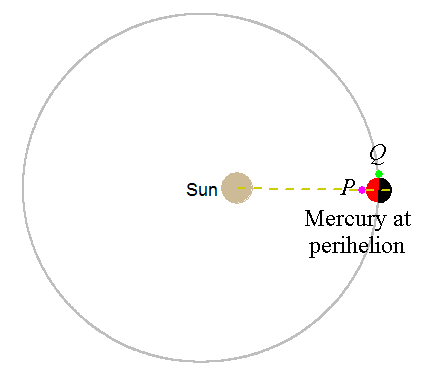
\includegraphics[width=7cm]{MercuryOrbit.png}
\caption{Mercur's orbit. The red region denotes the hemisphere facing the sun and 
is the day side. The black hemisphere is the night side.}
\label{fig:orbit}
\end{wrapfigure}

The purpose of this calculation is to visualize this approximate tidal locking. 
Consider two points $P$ and $Q$ at Mercury's equator. As shown in 
Figure~\ref{fig:orbit} where Mercury is at perihelion, $P$ faces the sun directly 
(``subsolar point'') and $Q$ is at an angle $\pi/2$ to the west of $P$. We will 
calculate the position of $P$ and $Q$ as a function of time as Mercury spins and revolves 
around the sun, and see how their relative angular positions with respect to the 
sun change with time. Since $Q$ is simply $\pi/2$ to the west of $P$, it suffices 
to compute the position of $P$. Mercury's spin axis tilts about $7^\circ$ with 
respect to its orbital angular momentum. However, the calculation ignores this 
small tilt. 

Animations are generated to show how the positions of $P$ and $Q$ relative to the 
sun change with time.

\section{Computation Method} 

Set up a coordinate system when the sun is at the origin and $\hat{x}$
points to the perihelion point. Let $\theta$ be the true anomaly of Mercury,
$\phi$ be the phase angle of point $P$ measured from the $\hat{x}$ direction and
$H$ be the hour angle of the sun as seen from point $P$ (see Figure~\ref{fig:angles}).
It follows that $H=\pi + \phi - \theta$. Integer factors of $2\pi$ may be added 
to $H$ and so the expression 
\beq
  H = \phi - \theta - \pi
\label{eq:H}
\eeq
is also valid. This expression is adopted so that $H=0$ at the configuration 
shown in Figure~\ref{fig:orbit} with $\theta=0$. If Mercury were tidally locked, 
$H$ would be time independent. The rate of change of $H$ is therefore a measure of 
the degree of tidal locking, and it is simply the difference of the rotational 
angular velocity and orbital angular velocity:
\beq
  \dot{H} = \dot{\phi} - \dot{\theta} = \frac{2\pi}{\prot} - \frac{2\pi a^2 \sqrt{1-e^2}}
{r^2 \porb} = \frac{2\pi}{\porb}\left( \frac{3}{2} - \frac{a^2 \sqrt{1-e^2}}{r^2} \right)
\label{eq:Hdot1}
\eeq

\begin{wrapfigure}{r}{7cm}
\vskip -5mm
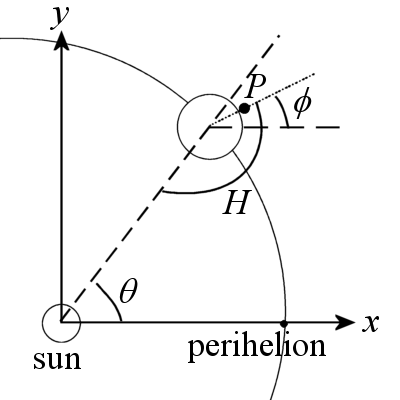
\includegraphics[width=7cm]{angles.png}
\caption{Hour angle $H$, true anomaly $\theta$ and phase angle $\phi$. The sizes
of Mercury, sun and Mercury's orbit are not drawn to scale.}
\label{fig:angles}
\end{wrapfigure}

Assume that $t=0$ is the configuration shown in Figure~\ref{fig:orbit}. 
The phase angle is simply given by 
\beq
  \phi(t) = \pi + \Omega_{\rm rot} t = \pi + \frac{2\pi t}{\prot} 
= \pi + \frac{3\pi t}{\porb} .
\label{eq:phi}
\eeq
The true anomaly can be determined by solving Kepler's equation 
\beq
  E - e \sin E = M = \frac{2 \pi t}{\porb} ,
\label{eq:kepler}
\eeq
where $E$ is the eccentric anomaly and $M$ is the mean anomaly. Mercury's 
center position $(x,y)$ is given by 
\beq
  x = a (\cos E - e) \ \ \ , \ \ \ y = a \sqrt{1-e^2}\, \sin E 
\label{eq:pos}
\eeq
and $\theta$ is the argument of the complex number $x+ yi$. Alternatively, 
$\theta$ can be computed by 
\beq
   \tan \frac{\theta}{2} = \sqrt{ \frac{1+e}{1-e}} \, \tan \frac{E}{2} .
\eeq
The distance from the sun is $r=\sqrt{x^2+y^2} = a (1-e \cos E)$. Substituting
this equation to~(\ref{eq:Hdot1}) gives 
\beq
  \dot{H} = \frac{2\pi}{\porb}\left[ \frac{3}{2} - \frac{\sqrt{1-e^2}}{(1-e\cos E)^2} 
\right] .
\label{eq:Hdot2}
\eeq

So here is the recipe: for any given time $t$, compute the phase angle $\phi$ 
using~(\ref{eq:phi}) and solve the Kepler equation~(\ref{eq:kepler}) 
for $E$. Next compute Mercury's position using~(\ref{eq:pos}) and calculate the 
true anomaly $\theta$. The position of $P$, $(x_P,y_P)$, is given by 
\beq
  x_P = x + R \cos \phi \ \ \ , \ \ \ y_P = y + R \sin \phi ,
\eeq
where $R$ is Mercury's radius. These quantities are sufficient to draw 
the configuration at time $t$. The hour angle $H$ and its time 
derivative can also be computed using~(\ref{eq:H}) and (\ref{eq:Hdot1}) 
[or (\ref{eq:Hdot2})].

It should be noted that it is actually not necessary to solve the transcendental 
equation~(\ref{eq:kepler}), as $x$, $y$, and $t$ can be parametrized 
by the eccentric anomaly $E$, i.e.\ $x=x(E)$, $y=y(E)$, and $t=t(E)$. 
One may choose to use $E$ as the independent variable in the calculation 
instead. However, if one wants to make $t$ uniformly spaced, which is 
useful if one wishes to make movies, the spacing in $E$ needs to be 
chosen appropriately. This is not too difficult for small time spacing 
$\Delta t$ since it follows from~(\ref{eq:kepler}) that 
\[
  \Delta E \approx \frac{2 \pi}{(1-e\cos E) \porb} \Delta t .
\]
A uniform time spacing can be created approximately by using
this particular $\Delta E$. However, solving the Kepler equation 
numerically is rather straightforward and was adopted in 
our calculation.

\section{Result}

\begin{center}
\begin{figure}
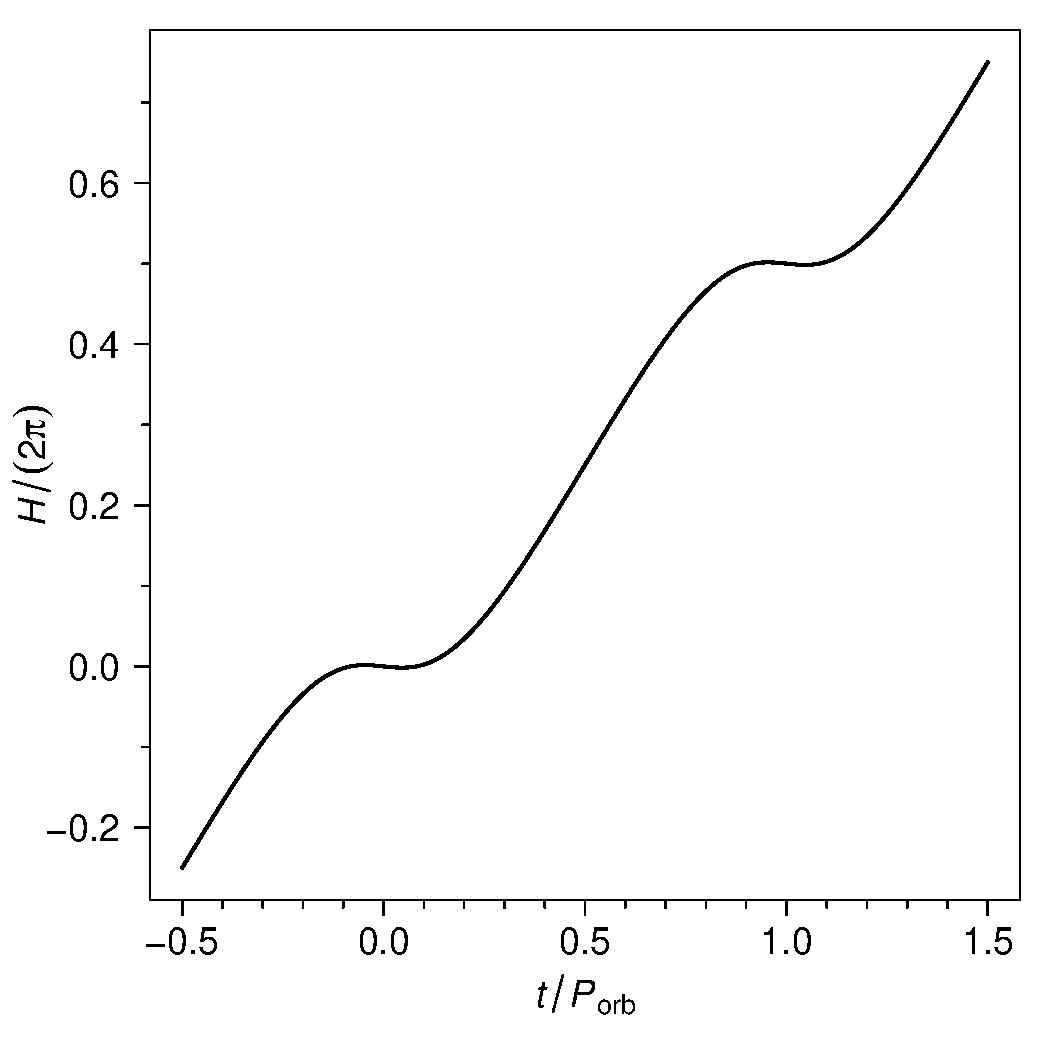
\includegraphics[width=8cm]{HourAngle.pdf}
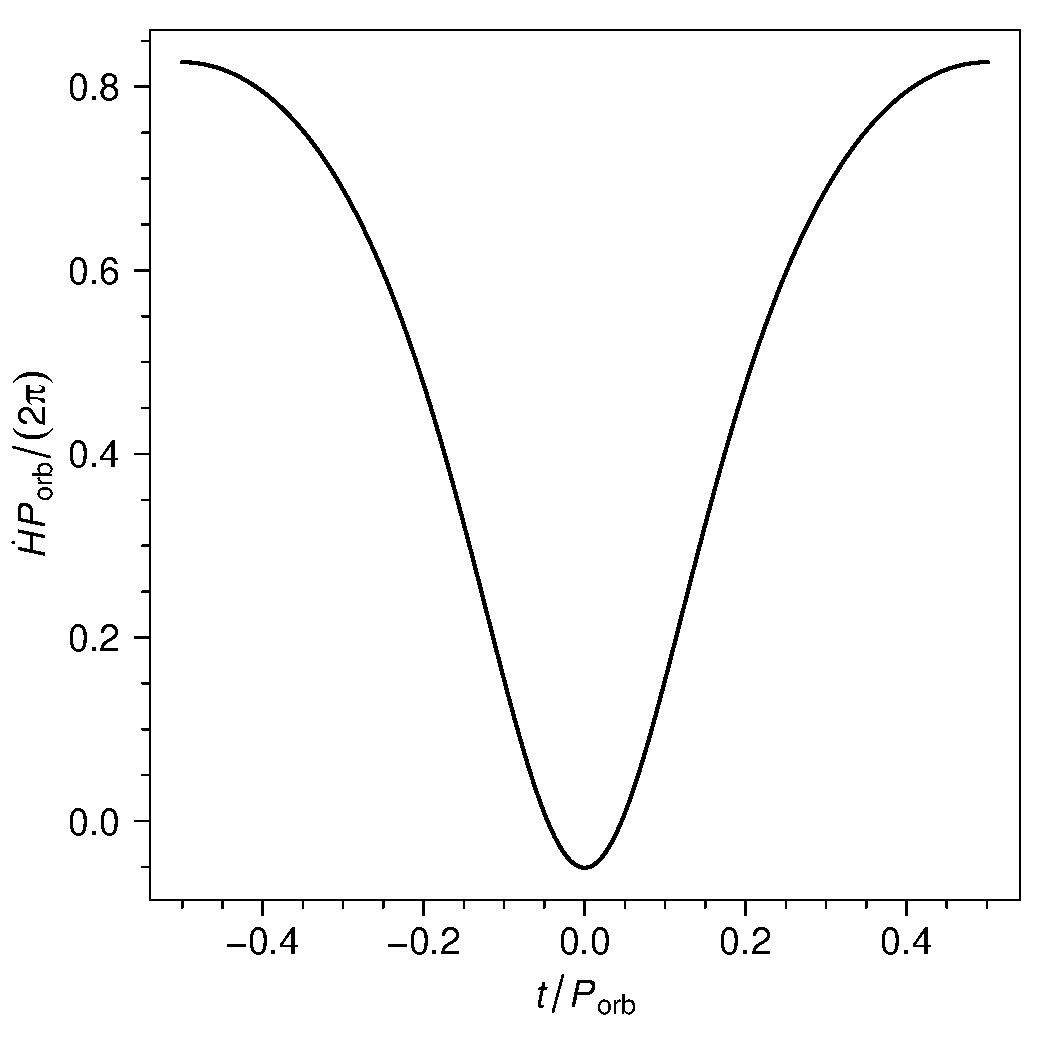
\includegraphics[width=8cm]{Hdot.pdf}
\caption{Left: Hour angle $H$ of the sun as seen at point $P$ (the 
magenta point in Figure~\ref{fig:orbit}) as a function of time. 
Right: The time derivative of $H$ as a function of time.}
\label{fig:H-Hdot}
\end{figure}
\end{center}

Choose $t=0$ to be the configuration in Figure~\ref{fig:orbit}. 
Figure~\ref{fig:H-Hdot} shows $H$ and $\dot{H}$ as a function of 
time as seen from the point $P$ (the magenta point in Figure~\ref{fig:orbit}). 
We see that there is a significant amount of time when $H$ remains nearly 
constant, an indication of approximate tidal locking. The $\dot{H}$ curve 
also shows the amount of time around the perihelion where $\dot{H} < 0$. 
Recall that $\dot{H} < 0$ means the sun's motion is eastward relative 
to horizon as seen in Mercury's sky. 

Data from the calculation show that $\dot{H} < 0$ when 
$-0.046 < t/\porb < 0.046$. Since $\porb = 87.969$ (Earth) days, the retrograde 
motion lasts about 8 days. During this period, the hour angle has changed by 
$\Delta H = -0.0194$ radians. For comparison, the angular radius of the sun 
as seen on Mercury at $|t| < 0.046 \porb$ is about 0.015 radians. At point $P$, 
the sun is high near the zenith. However, at point $Q$ which is $\pi/2$ to 
the west of $P$ (see Figure~\ref{fig:orbit}), the sun hovers about the 
horizon during this period. 

It is interesting to analyze the sun's positions as seen from $Q$. 
The hour angle of the sun at $Q$, $H_Q$, is related to $H$ by 
$H_Q = H - \pi/2$. Sunrise is defined as the moment when the sun's 
upper edge touches the horizon. Since Mercury doesn't have an atmosphere, 
we don't need to correct for atmospheric refraction as on Earth. Sunrise 
occurs when $H_Q = -\pi/2 - \alpha_\odot$ or $H=-\alpha_\odot$, where 
$\alpha_\odot = R_\odot / r$ is the angular radius of the sun and 
$R_\odot = 6.955\times 10^8$~m is the solar radius. Calculation shows 
that sunrise occurs around $t=-0.1 \porb$ and the angular radius of the 
sun is $\alpha_\odot = 0.014 {\rm rad} = 0.8^\circ$. At $t=-0.046\porb$, 
the sun's center is 0.0097~radians ($0.56^\circ$) above the horizon and the 
lower edge of the sun is still below the horizon. The sun then moves 
backward in the sky and is now setting. At $t=0.046 \porb$, the sun's center 
is 0.0097 radians ($0.56^\circ$) below the horizon but the upper edge of the 
sun is still above the horizon. The sun rises again as $\dot{H}>0$. The lower 
edge of the sun touches the horizon at $t=0.1\porb$. Hence the whole sunrise 
lasts $0.2\porb$ or 17.6 days as seen at $Q$. Although an observer at $Q$ 
sees the upper edge of the sun above the horizon during this period, observers 
at some points further west of $Q$ will first see the sun rise, but 
before the whole sun rises it sets and 
rises again later when Mercury moves further away from the perihelion.

\begin{figure}
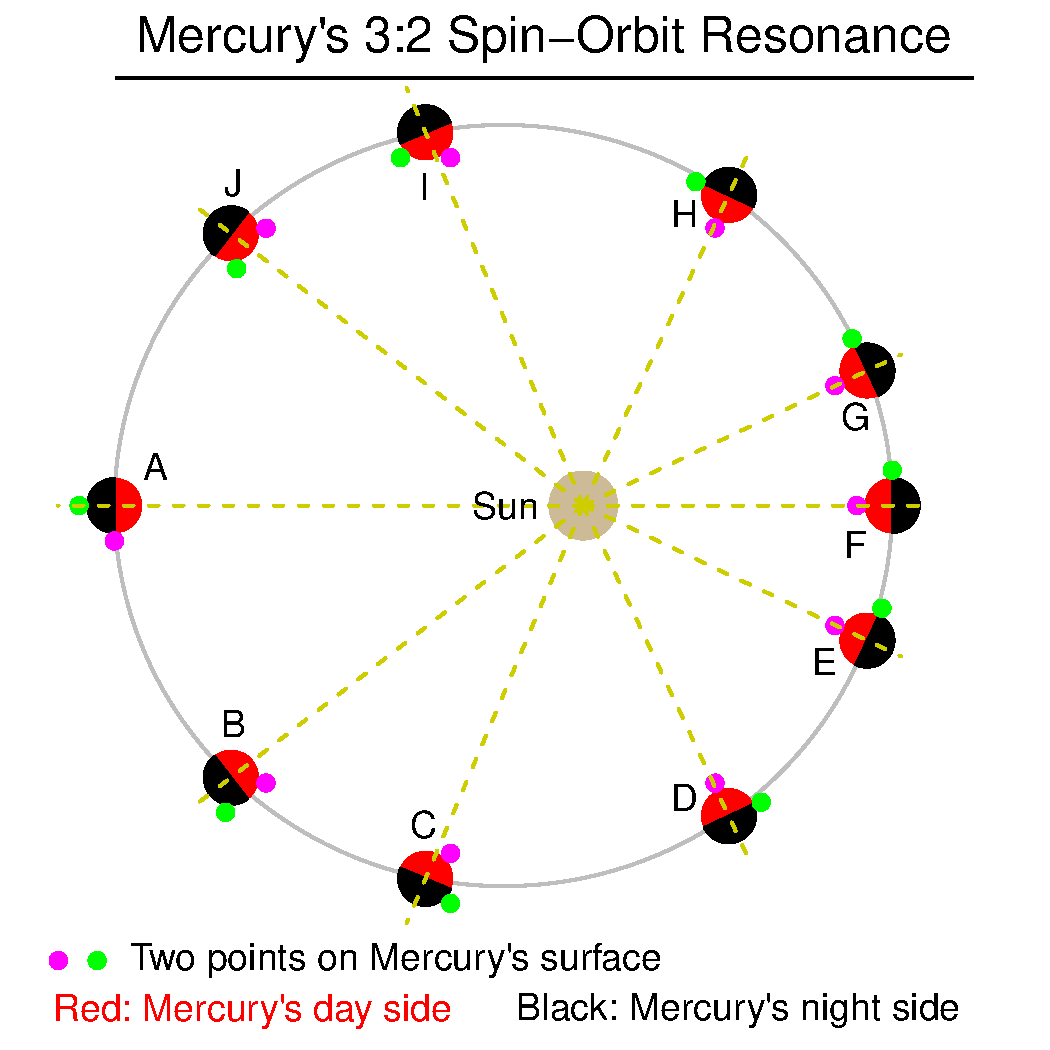
\includegraphics[width=15cm]{SpinOrbit.pdf}
\caption{Mercury's spin-orbit configuration at various times in its orbit. 
The times from points A--J are $t/\porb =$-0.5, -0.35, -0.25, -0.125, -0.046, 
0, 0.046, 0.125, 0.25, and 0.35. The magenta and green points are the same points 
$P$ and $Q$ shown in Figure~\ref{fig:orbit}. Red hemisphere is Mercury's 
day side and black hemisphere is the night side. 
The sun's motion relative to horizon is eastward from points E to G. Approximate 
tidal locking occurs from points D to H, where the hour angle 
changes by $\Delta H = 0.06$ radians (about $5^\circ$) only. 
The configurations are periodic with the synodic period equal to 
$2\porb$. The configurations for $0.5 < t/\porb < 1.5$ can be 
obtained from the configurations at time $t-\porb$ by simply 
putting the magenta and green points to the opposite side of 
Mercury.}
\label{fig:configs}
\end{figure}

Figure~\ref{fig:H-Hdot} suggests that the period when $H$ is nearly constant 
lasts longer than the period when $\dot{H}<0$. Exactly how long it is 
depends on the criterion of ``nearly constant.'' For $-0.114 < t/\porb < 0.114$, 
$-0.03 < H < 0.03$. For $-0.125 < t/\porb < 0.125$, $-0.045 < H < 0.045$. 
Hence for a quarter of orbital period around perihelion, or 22 (Earth) days, 
the sun remains less than $2.6^\circ$ from the zenith as seen from $P$. 
This gives us an idea of the degree of tidal locking near perihelion.

Finally, Figure~\ref{fig:configs} shows the configurations of Mercury 
at various times of the orbit. Two animations have been created to show 
the spin and orbit motions. One animation shows the configurations displayed in Figure~\ref{fig:configs} 
as a function of time. The other one shows the change of day-night boundary 
as a function of time as seen in a frame corotating with Mercury.
In the animations, however, the time is shifted by $0.5 \porb$, 
i.e. $t({\rm animation}) = t - 0.5 \porb$. So $t({\rm animation})=0$ corresponds 
to Mercury at aphelion. The shift is made in order to see the occurrence of approximate tidal 
locking when Mercury moves close to the perihelion. If the animations start at Mercury 
at perihelion, we will miss the beginning of the approximate tidal locking and will 
have to wait until Mercury completes one orbit.

\end{document}
